\documentclass[hyperref={pdfpagelabels=false}]{beamer}
\usepackage{graphicx,lmodern,subfigure,ulem,color,graphicx,tikz,booktabs,natbib}
\usepackage{mathrsfs}
\usetheme{Warsaw}
%\definecolor{beamer@blendedblue}{rgb}{0.1,0.5,0.1}
%\definecolor{ForestGreen}{RGB}{60, 140, 60}
%\setbeamercolor{structure}{fg=beamer@blendedblue}
\setbeamertemplate{navigation symbols}{}
\setbeamertemplate{footline}[frame number]
\bibliographystyle{chicago}
\newcommand{\spitem}{\vspace{.3cm}\item}
\newcommand{\elas}{$E_{labor}$}
%\def \FigPath {Users\th3\Documents\Job_Market_Paper\Code\Figures} 


\title{Uncertainty Shocks and Financial Shocks}
\author{Marco Brianti}
\institute{Boston College}
\date{September 2018}


\begin{document}
	
	\frame{\titlepage \begin{center} Dissertation Project \end{center} }
	

\frame{\frametitle{Credit Conditions and Uncertainty (I)}


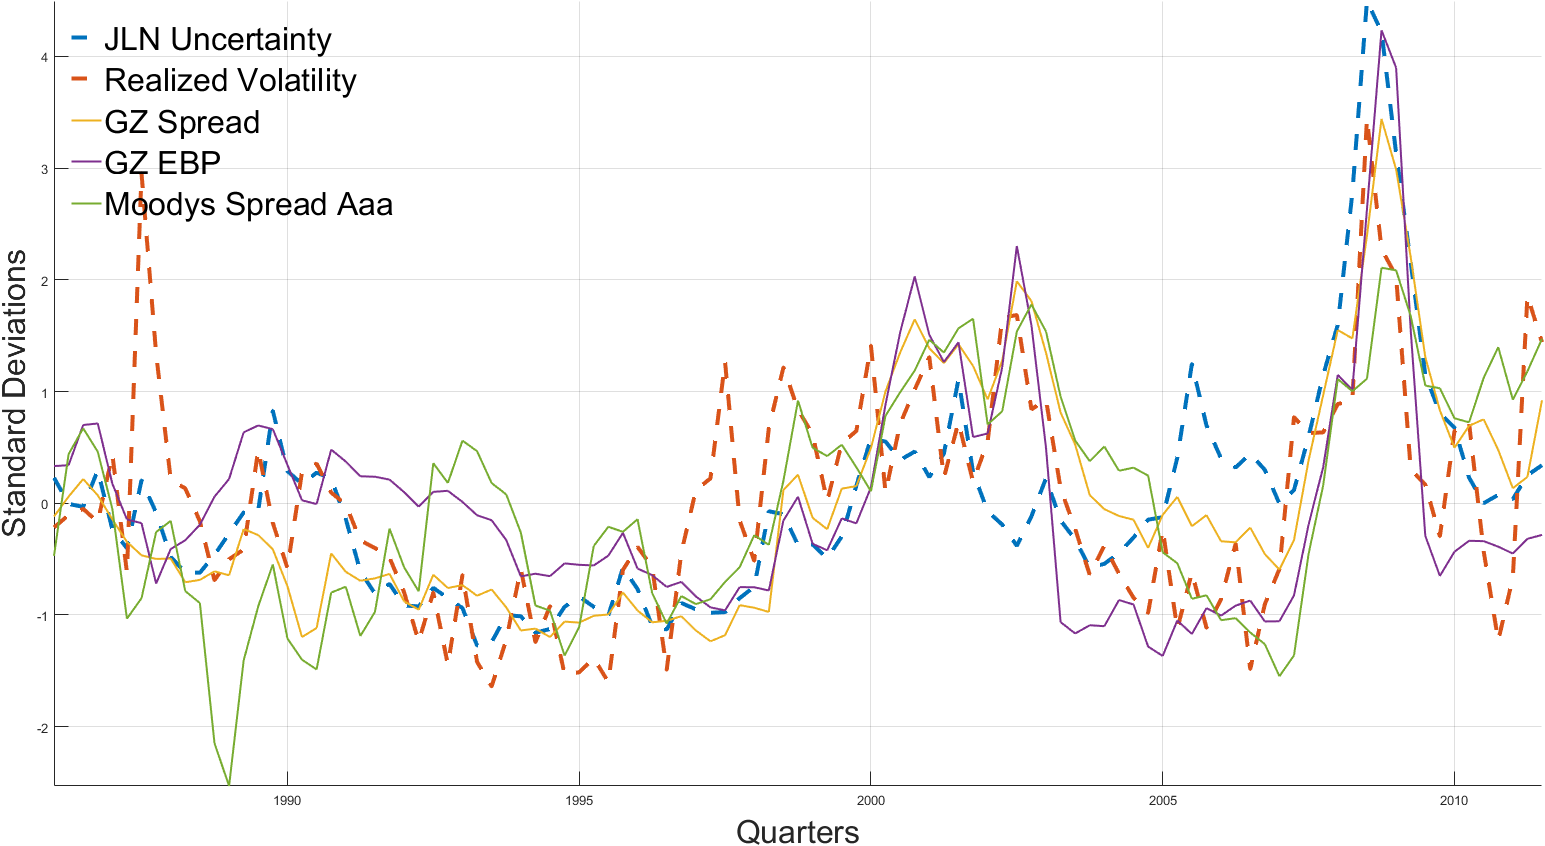
\includegraphics[scale=0.26]{Financial_Uncertainty}

\

Proxies for \textbf{credit conditions} and \textbf{uncertainty} are both countercyclical and tightly correlated.

}


\frame{\frametitle{Credit Conditions and Uncertainty (II)}
	
	
	\begin{table}
		\begin{tabular}{c||cccccc}
            & JLN         &      RV    & GZ  & EBP &    Moodys Aaa 	  \\
            \hline
            \hline
JLN	        &    1        &       -    &      -     &       -    &    -   \\
RV        	&    0.5865   &  1         &     -      &     -      &    -   \\ 
GZ       	&    0.7742   &  0.6247    &  1         &     -      &     -  \\
EBP      	&    \textbf{0.6213}   &  0.5621    &  0.7316    &  1         &     -  \\
Moodys Aaa	&    0.4386   &  0.4554    &  0.7993    &  0.5243    &    1   \\
	\end{tabular}
	\end{table}

\

\

As suggested by the graph above, all the variables are strongly correlated.

}


\frame{\frametitle{Financial Shocks and Uncertainty Shocks}
	
	Stock and Watson (2012); Caldara et al. (2016) among others shown that uncertainty shocks and financial shocks are deeply confounded.
	
	\
	
	\
	
	
	$$
	corr(\iota^{EBP}_t,\iota^{JLN}_t) \approx 0.45
	$$
	
	\
	
	\
	
	
	where $\iota^{EBP}_t$ is an unpredictable innovation in the \textbf{excess bond premium} from Gilchrist and Zakrajzek (2012) and $\iota^{JLN}_t$ is an unpredictable innovation in the \textbf{uncertainty proxy} from Jurado et al. (2015).
	

	

	
	
	
}

\frame{\frametitle{Both a theoretical and empirical question}

	Literature did not succeed yet to disentangle the two exogenous sources for two main reasons:
\begin{enumerate}
	\item Simultaneity
	\begin{itemize}
		\item Both types of variables are fast moving
				\end{itemize}	
			\item Effect on observables
			
			\begin{itemize}
			\item They have the same qualitative effects on prices and quantities
\end{itemize}
\end{enumerate}

\

\

As a result, both \textbf{zero-impact restrictions} cannot be used and \textbf{internal instruments} are not available.
	
}

\frame{\frametitle{My contribution}
	
	I want to take a step back and show evidence and theory that financial and uncertainty shocks
	
	
	\begin{itemize}
		
		\item are not \textbf{qualitatively equivalent}, and
	
		
		\item they can be \textbf{successfully disentangled}.
		
		\end{itemize}
	
	\	
	
	
	
	In particular, 
	
	\
	
	
	\begin{enumerate}
\item	I will show evidence that there exists a set of variables which respond differently to financial and uncertainty shocks. 
	\begin{itemize}
		\item there exists an \textbf{economic intuition} for this response
		\item those variables can be used as \textbf{internal instruments}
	\end{itemize}

\

\item I will provide a \textbf{new econometric method} to use internal instruments to disentangle two structural shocks.

\end{enumerate}
}
	


\frame{\frametitle{Economic Intuition - Partial Equilibrium Analysis (I)}
	
	Effect of a financial shock: 
	
	\begin{figure}[plain]
		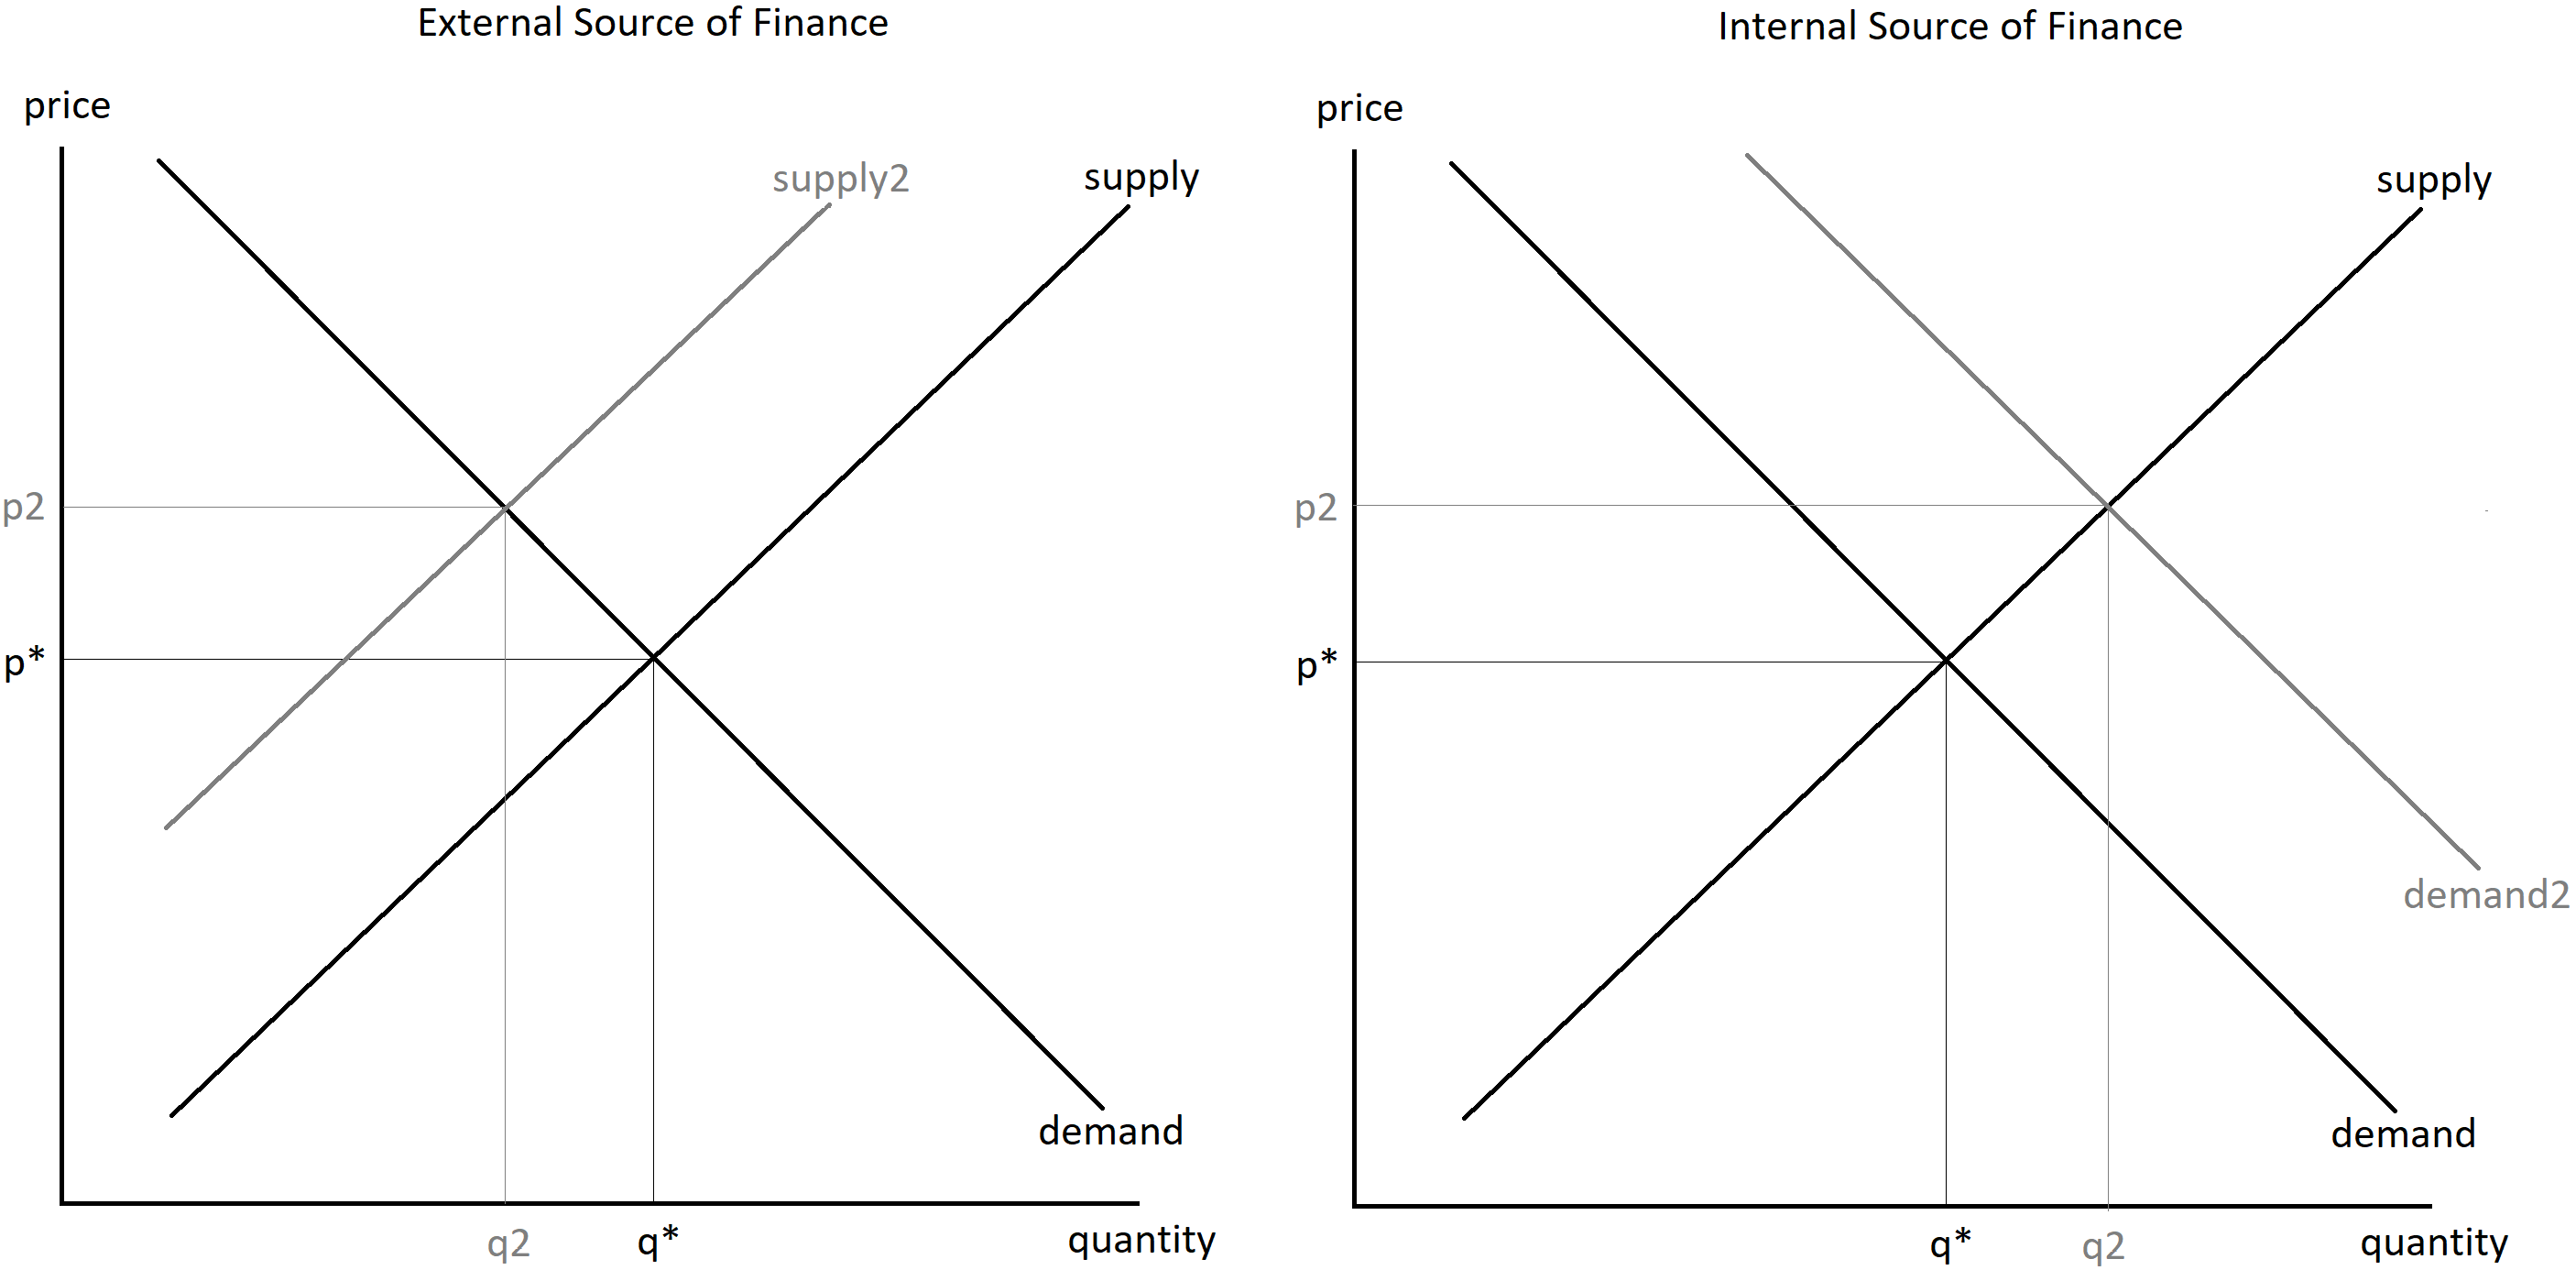
\includegraphics[scale=0.13]{fig_financial_supply_demand_F}
	\end{figure}
	
	Notice that I am taking as given the supply of internal source of finance. 
}

\frame{\frametitle{Economic Intuition - Partial Equilibrium Analysis (II)}
	
	Effect of an uncertainty shock: 
	
	\begin{figure}[plain]
		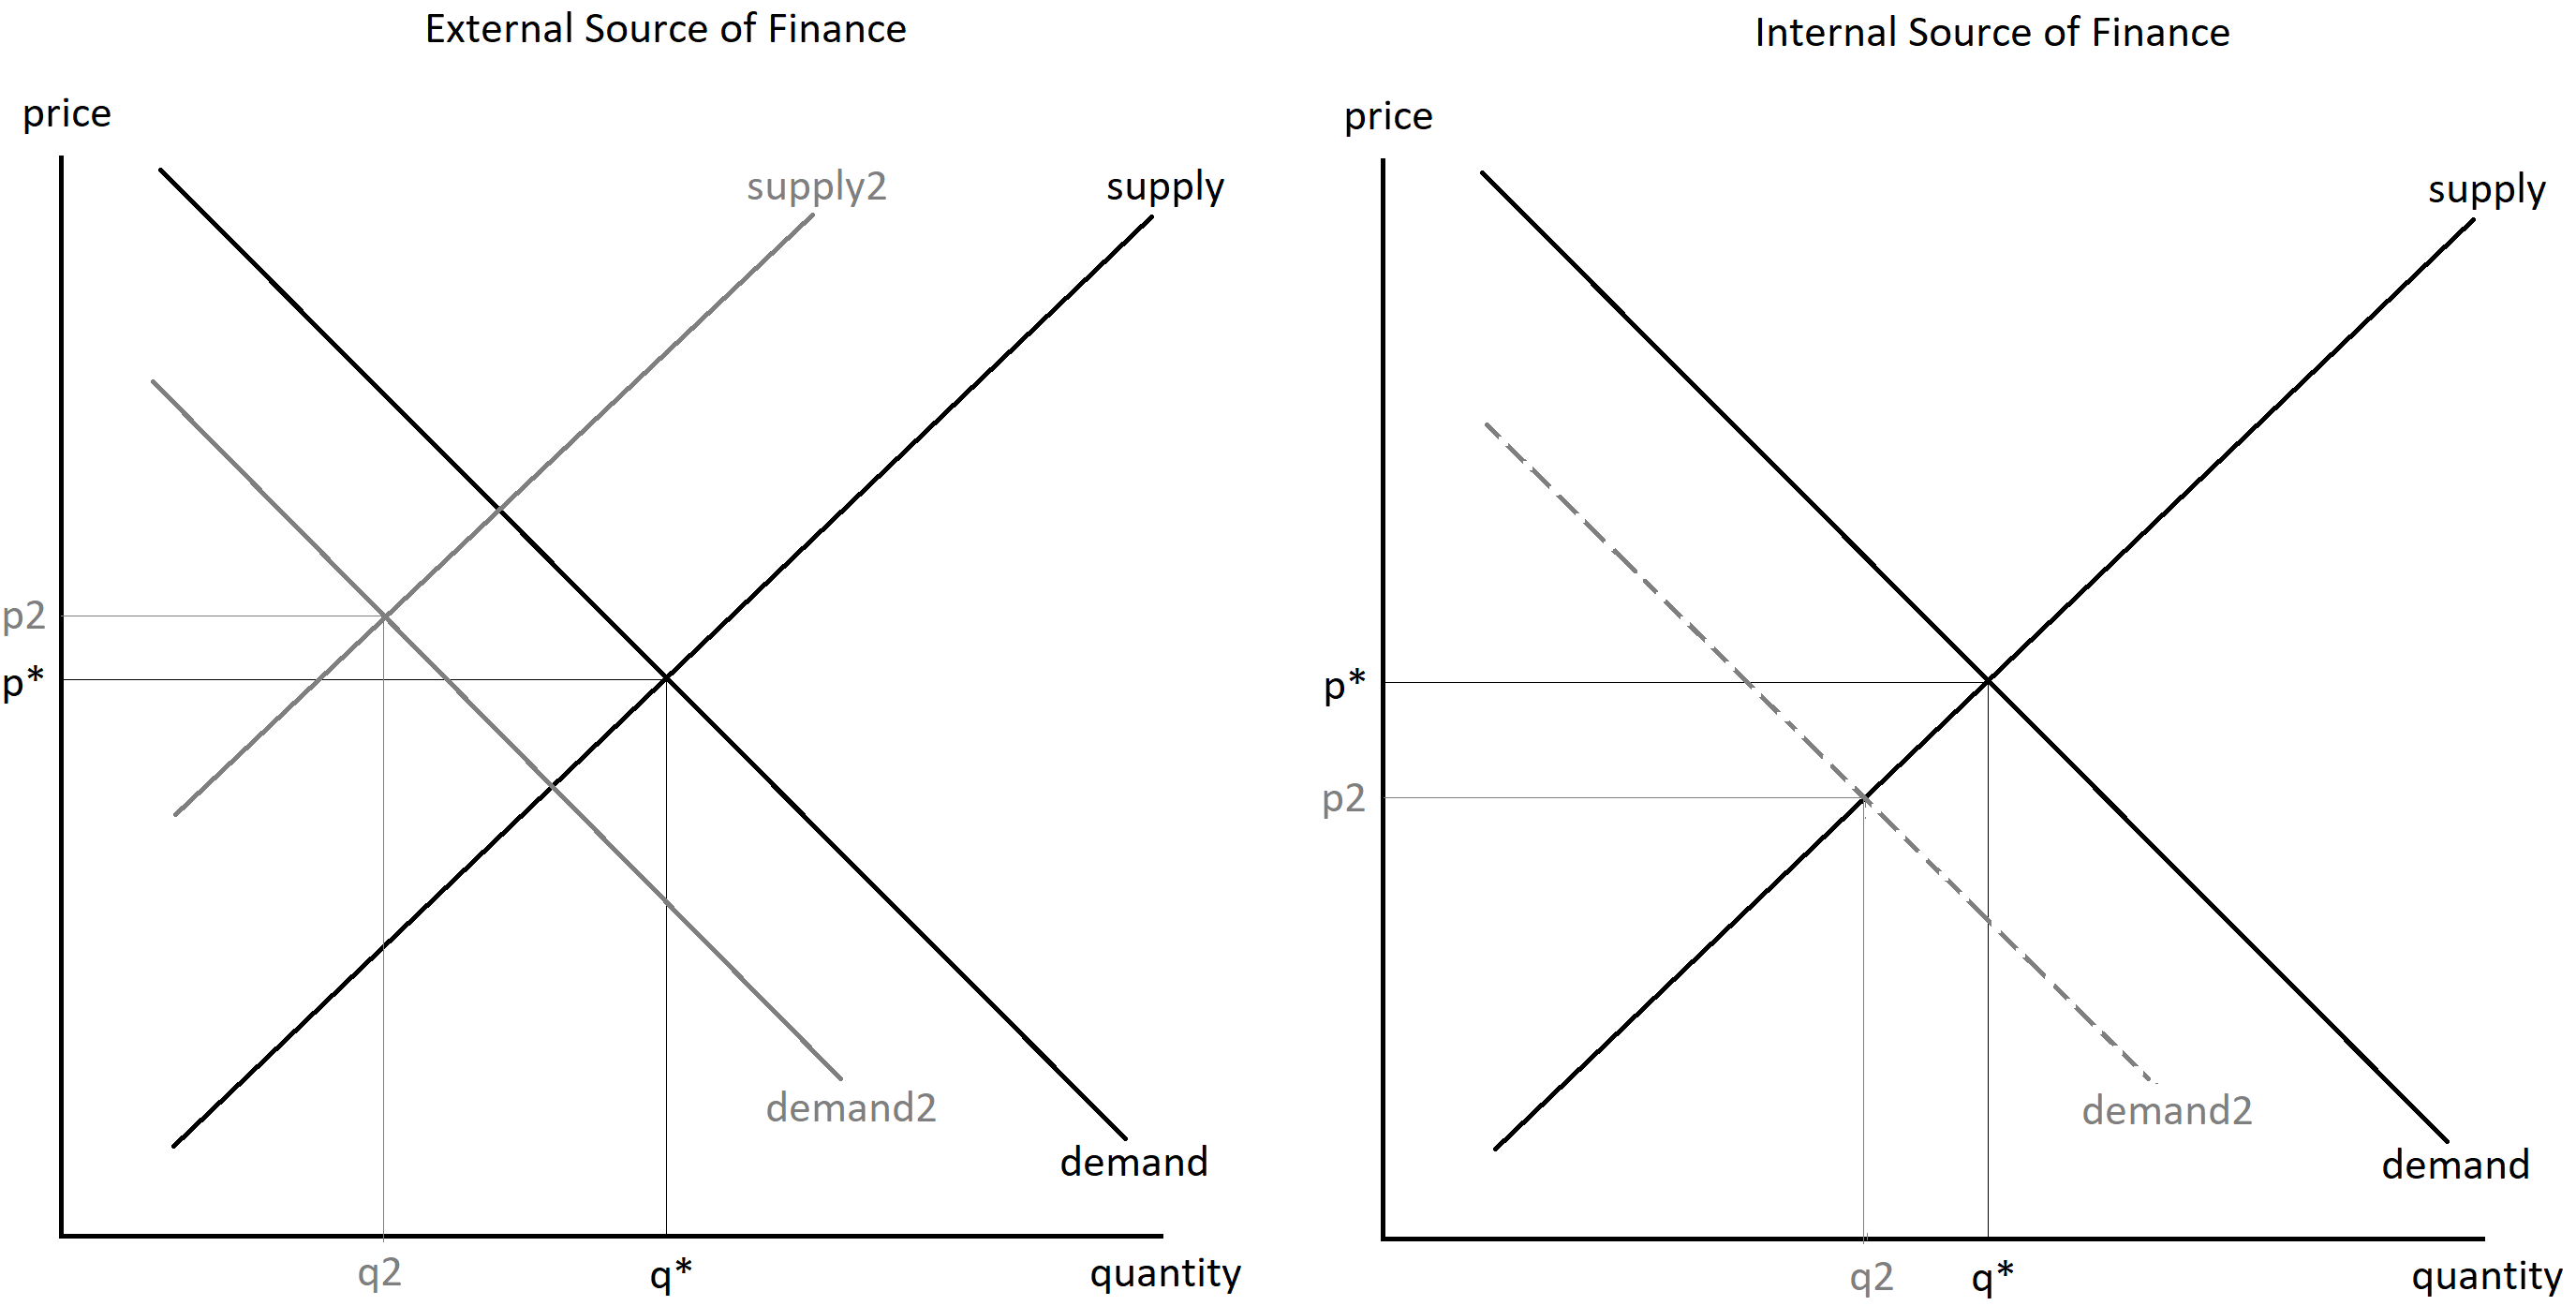
\includegraphics[scale=0.13]{fig_financial_supply_demand_U}
	\end{figure}
	
	Notice that I am taking as given the supply of internal source of finance. 
	
}


\frame{\frametitle{Economic Intuition}
	
	
	\begin{itemize}
		
		\item 	After a \textbf{decrease in credit supply} - for a given supply of internal funds - quantity of the internal source of finance should increase.
		
		\begin{itemize}
			\item On impact, firms do not invest because they are \textbf{financially constrained}.
			\item Bernanke, Gertler, and Gilchrist, 1999; Jermann and Quadrini, 2012.
		\end{itemize}
		
		
		\
		
		\item After an \textbf{increase in uncertainty} - for a given supply of internal funds - quantity of the internal source of finance should either decrease or remain unchanged.
		
				\begin{itemize}
			\item \textbf{Real-options effects} imply that during period of uncertainty firms opt for wait-and-see rather than investing.
			\item Bernanke, 1983; Brennan and Schwartz, 1985; McDonald and Siegel, 1986.
		\end{itemize}
		
	\end{itemize}
	
}

		\frame{\frametitle{Variables of Interest by Bureau of Economic Analysis}
	
	\textbf{Cash Flow} is a profit-related measure of \textbf{internal funds} available for investment. [The NIPA Handbook, December 2015]
	
	\

	\begin{itemize}
		\item[ ] Corporate Profits
		\item[$-$] Dividends
		\item[$+$] Consumption of Fixed Capital
		\item[$-$] Net Capital Transfers Paid  
		\item[$=$] \textbf{Cash Flow}
		\end{itemize}


	\
	
	where 
	
	\begin{enumerate}
		\item \textbf{consumption of fixed capital} is capital depreciation
		\item \textbf{net capital transfers paid} are unrequited transfers associated with the acquisition or disposal of assets.
	\end{enumerate}
	

	

	
}
	
	
	\frame{\frametitle{Controlling for the Supply of Internal Funds}	
		
		The main source (\textbf{supply}) of internal funds available for investment is \textbf{corporate profits} of the current period.
		
		\
		
		Not surprisingly, profits are \textbf{procyclical} implying that the supply of internal funds cannot be taken as given.
		
		\
		
		
		In order to control for \textbf{general equilibrium effect}, cash flow needs to be normalized by the corporate profit.
		
		\
		
		As an intuition, cash flow over profits is an \textbf{index} between $0$ and $1$
		\begin{itemize}
			\item If the index is equal to zero, current profits are fully distributed outside the firm
			\item If index is equal to one, current profits are going to be fully used inside the firm
		\end{itemize}
		
	}

\frame{\frametitle{From Theory to Data}
	
Partial equilibrium analysis suggests that

\begin{itemize}
	\item Normalized cash flow should \textbf{increase} after a \textbf{financial shock}
	\begin{itemize}
	\item[$\Rightarrow$] Firms focus on different source of finance because financially constrained 
	\end{itemize}
	\item Normalized cash flow should \textbf{not increase} after an \textbf{uncertainty shock}
	\begin{itemize}
		\item[$\Rightarrow$] Demand for any source of finance decrease together with the supply
	\end{itemize}
\end{itemize}	

\

\

Using aggregate US data I run a 2-step regression in favor of previous analysis.
	
	
	
}
	

\frame{\frametitle{Step 1}
	
	Regress both a proxy for uncertainty and financial conditions on lagged principal components obtained from a large dataset,
	\begin{itemize}
		\item $F_t = \alpha^F + A_F(L)PC_{t-1} + \iota^F_t$
		\item $U_t = \alpha^U + A_U(L)PC_{t-1} + \iota^U_t$
	\end{itemize}

where 

\begin{itemize}
	\item $F_t$ is a proxy of financial conditions
	\item $U_t$ is a proxy of uncertainty
	\item $PC_t$ is a vector of principal components
\end{itemize}

\

Goal is to obtain $\iota^F_t$ and $\iota^U_t$ as \textbf{unforecastable components} of $F_t$ and $U_t$, respectively.

}

\frame{\frametitle{Step 2}
	
Regress normalized cash flow on both innovations $\iota^F_t$ and $\iota_t^U$, controlling for its forecastable part,
	
	$$
	\tilde{CF}_t = \alpha + B(L)PC_{t-1} + \beta^{F} \iota_t^F + \beta^{U} \iota_t^U + \varepsilon_t
	$$
	
	where $\tilde{CF}_t$ is cash flow normalized by corporate profits.
	
	\
	
	\
	
	\textbf{Results.}
	
	\begin{itemize}
		\item $\beta^F$ is always \textbf{positive} and \textbf{significant} at $1$\%.
		
		\item $\beta^U$ is almost always \textbf{not significant}. 
	\end{itemize}


	
}

	
	\frame{\frametitle{Robustness Checks}
		
\begin{itemize}
	\item Changing the number of lags, ranging from $3$ to $6$
	\item Changing the number of $PC_t$, ranging from $4$ to $8$
	\item Adding different controls in both steps
	\item Using different measures of uncertainty and credit supply
\end{itemize}

}

\frame{\frametitle{Penalty Functions}

Penalty functions is a constrained maximization problem where the importance of the constraint depends on a exogenously given coefficient.

\

Given a standard constrained maximization problem,
$$
\max_x f(x) \ \ \text{s.t} \ \ g(x) \geq 0
$$
a penalty function is
$$
\max_x f(x) + \delta g(x), \ \ \delta > 0
$$

\begin{itemize}
\item If $\delta = 0$ the constraint $g(x)$ is not taken into account
\item If $\delta \rightarrow \infty$ optimal solution maximizes constraint $g(x)$
\end{itemize}

}




\frame{\frametitle{Penalty Functions Approach (PFA) on Structural VARs}
	
	
Firstly presented by Uhlig (2005), PFA has the flavor of \textbf{sign restrictions} but with the advantage that the problem is just identified, delivering an \textbf{unique solution}.

\

\

\textbf{Shortcoming}: parameter $\delta$ is exogenously chosen making the identification strategy less credible.

\

\

I suggest a \textbf{general penalty function approach} for internal instruments where $\delta$ is treated as an endogenous parameter chosen by the data.

}

\frame{\frametitle{Step 1 - Identifying uncertainty shocks}

Given the reduced-form system $X_t = B X_{t-1} + \iota_t$ where 
\begin{itemize}
\item $X_t = [U_t \ \ F_t \ \ Y_t]'$ where $Y_t$ are macroeconomic variables.
\item $\iota_t' \iota_t = \Sigma_{\iota}$
\end{itemize}

\

\textbf{Step 1}
\begin{eqnarray*}
\max_{\gamma_{U}} \ & \ \sum_{t=0}^K e'_U B^t \tilde{A}_0 \gamma_U - \delta e'_{CF} \tilde{A}_0 \gamma_U \\
\text{subject to} \ & \ \delta \geq 0 \ \ \text{and} \ \ \gamma_U \gamma_U' = 1
\end{eqnarray*}
 where 
\begin{itemize}
	\item $\tilde{A}_0 \tilde{A}'_0 = \Sigma_{\iota}$
	\item $e_j$ is a selection vector of variable $j$
\end{itemize}

\

An uncertainty shock maximizes its effect on uncertainty over the first $K$ quarters with penalty $\delta$ if cash flow is positive on impact.
	
}

\frame{\frametitle{Step 2 - Identifying financial shocks}


Given the reduced-form system $X_t = B X_{t-1} + \iota_t$ where 
\begin{itemize}
	\item $X_t = [U_t \ \ F_t \ \ Y_t]'$ where $Y_t$ are macroeconomic variables.
	\item $\iota_t' \iota_t = \Sigma_{\iota}$
\end{itemize}

\

\textbf{Step 2}
\begin{eqnarray*}
	\max_{\gamma_{F}} \ & \ \sum_{t=0}^J e'_F B^t \tilde{A}_0 \gamma_F + \delta e'_{CF} \tilde{A}_0 \gamma_F \\
	\text{subject to} \ & \ \delta \geq 0, \ \ \gamma_F \gamma_F' = 1 \ \ \text{and} \ \ \gamma_U \gamma_F' = 0
\end{eqnarray*}
where 
\begin{itemize}
	\item $\tilde{A}_0 \tilde{A}'_0 = \Sigma_{\iota}$
	\item $e_j$ is a selection vector of variable $j$
\end{itemize}

\


A financial shock maximizes its effect on credit spread over the first $J$ quarters with penalty $\delta$ if cash flow is negative on impact.

}

\frame{\frametitle{How to choose $\delta$}
	
	Choose $\delta$ large enough such that it does not matter if you run Step 1 or Step 2 first.
	
	\
	
	In other words, internal instrument intervention should be strong enough such that $\gamma_U \gamma_F' \simeq 0$
	
	\
	
	Solution is \textbf{unique} over many dimensions.
	
}



















\end{document}